% \begin{frame}{Sixteen years of building-level insurance data}
%   \vspace{0.25cm}
%   \begin{columns}[T,onlytextwidth]
%     \begin{column}{0.40\textwidth}
%       \textbf{Insurance data from Gjensidige}
%       \begin{itemize}
%         \item One of Norway's largest insurers, roughly a quarter of
%           the market
%         \item NR and Gjensidige long-running relationship %
%           % TODO: Footnote with this article.
%         \item Three-way collaboration: Gjensidige, NR, and ECoCA
%       \end{itemize}
%     \end{column}
%     \begin{column}{0.57\textwidth}
%       % Replace with the English-labelled plot using the same filename.
%       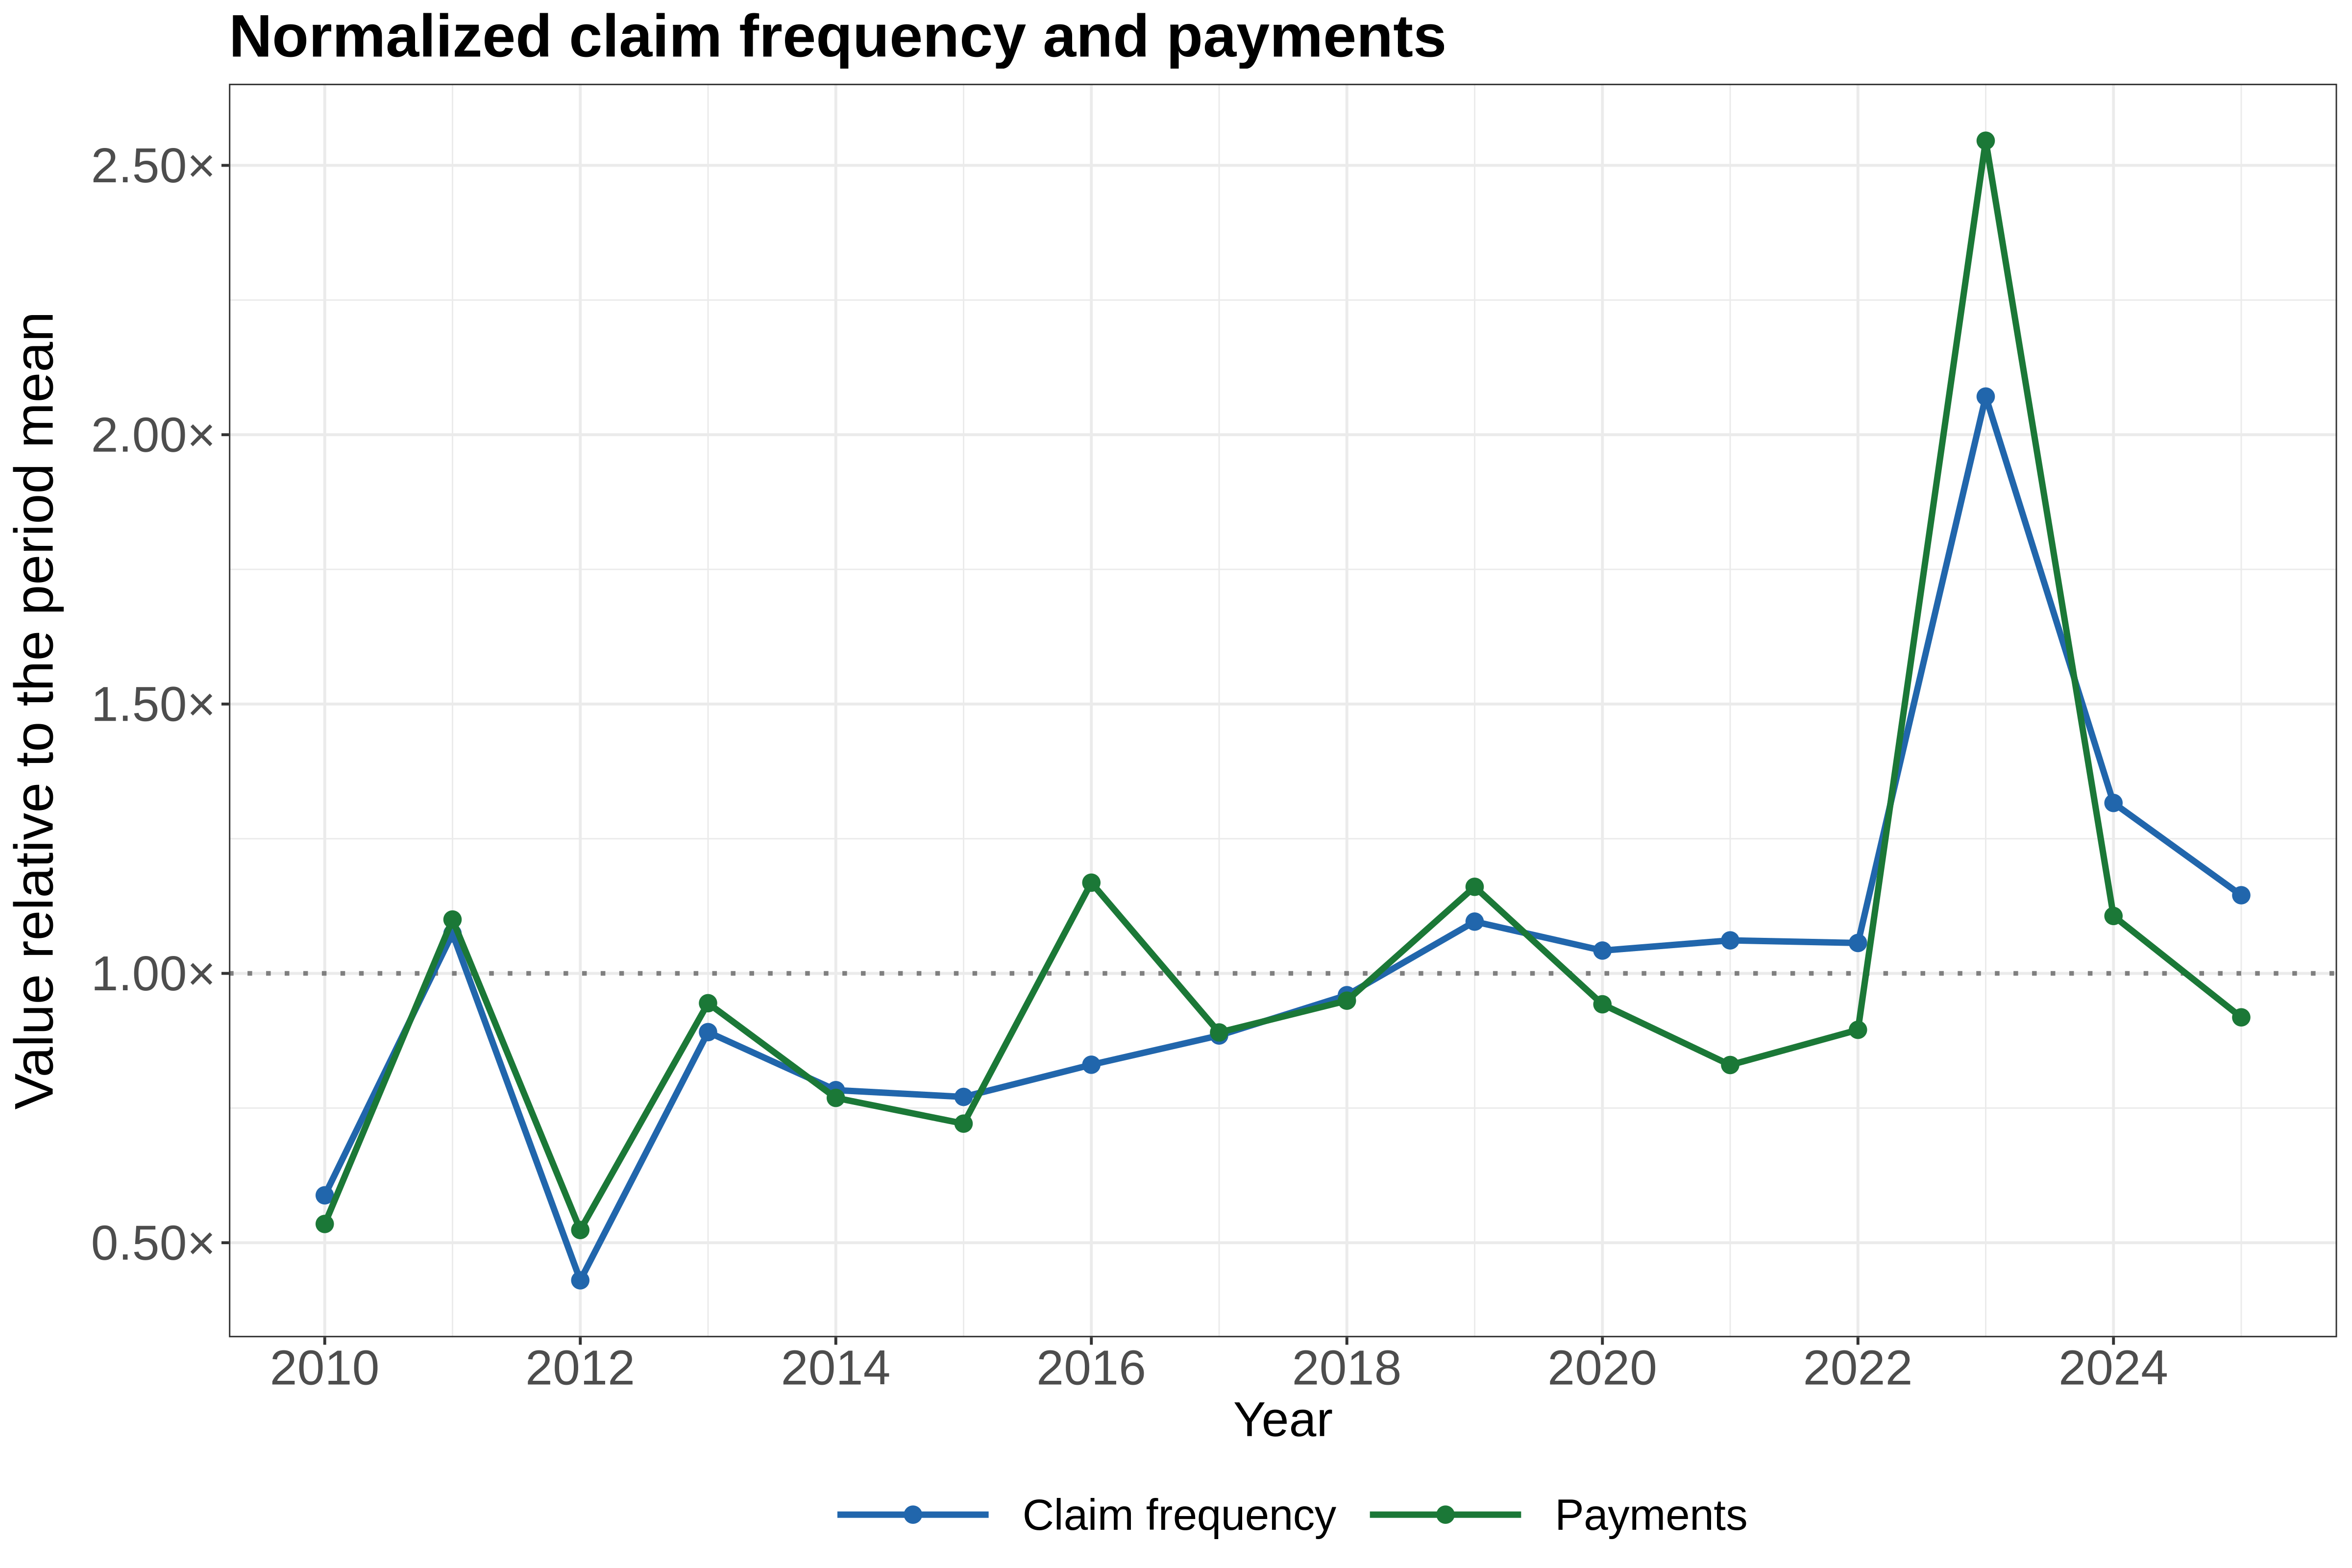
\includegraphics[width=\linewidth,height=0.60\textheight,keepaspectratio]{images/normalized_claim_frequency_and_payments.png}
%     \end{column}
%   \end{columns}
%   \sourceNote{Gjensidige building portfolio, 2010--2025}
% \end{frame}

% Say the parts from the above frame when presenting this slide,
% instead of using two slides to say almost the same thing.
\begin{frame}{Sixteen years of building-level insurance data}
  \vspace{0.25cm}
  \begin{columns}[T,onlytextwidth]
    \begin{column}{0.40\textwidth}
      \textbf{Gjensidige data, 2010--2025:}
      \begin{itemize}
        \item Daily claim registration and building-level exposure
        \item Claims, payouts, and deductibles
        \item On the order of 200k contracts, and 40k claims
        \item Several residential and commercial building types
          % \item Values inflation adjusted to 2026 NOK
          % NOTE: Claims below the deductible are not observed
      \end{itemize}
    \end{column}
    \begin{column}{0.57\textwidth}
      % Replace with the English-labelled plot using the same filename.
      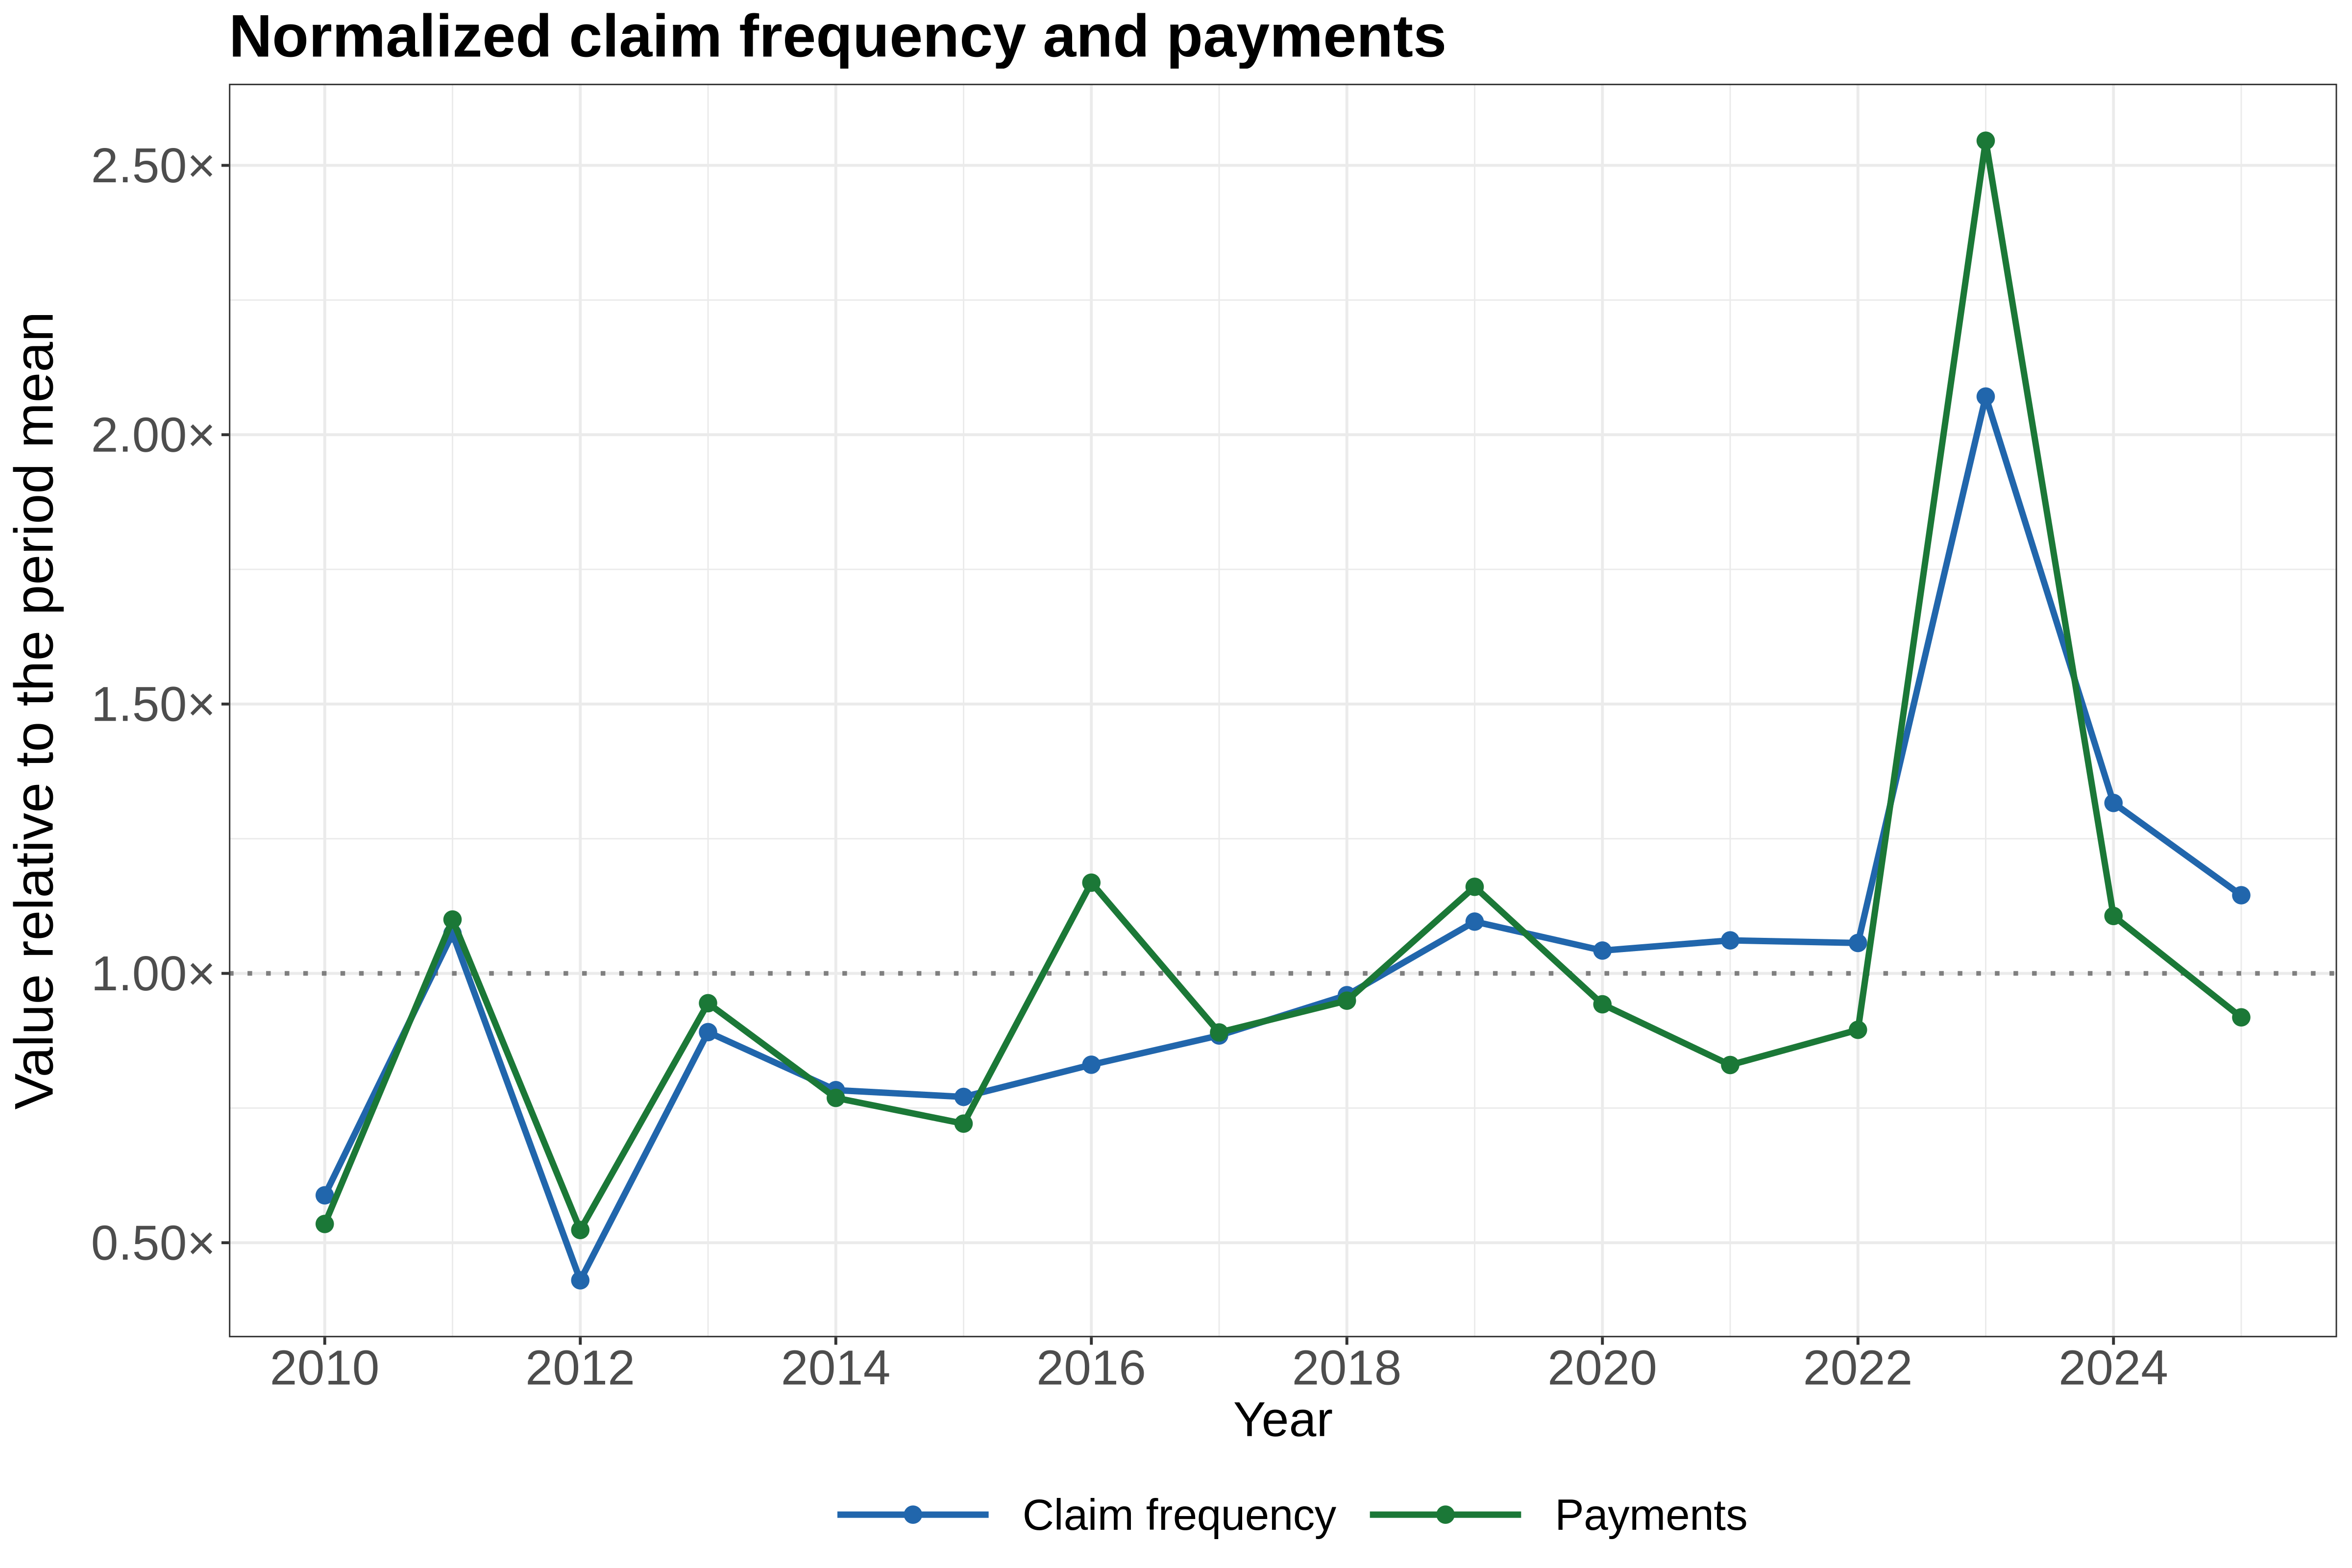
\includegraphics[width=\linewidth,height=0.60\textheight,keepaspectratio]{images/normalized_claim_frequency_and_payments.png}
    \end{column}
  \end{columns}
  \sourceNote{Gjensidige building portfolio, 2010--2025}
\end{frame}

\begin{frame}{Topographic data sources}
  \vspace{-0.1cm}
  \begin{columns}[T,onlytextwidth]
    \begin{column}{0.49\textwidth}
      \centering
      \hspace{-1.2cm}
      Topographic wetness index (TWI)\\[0.08cm]
      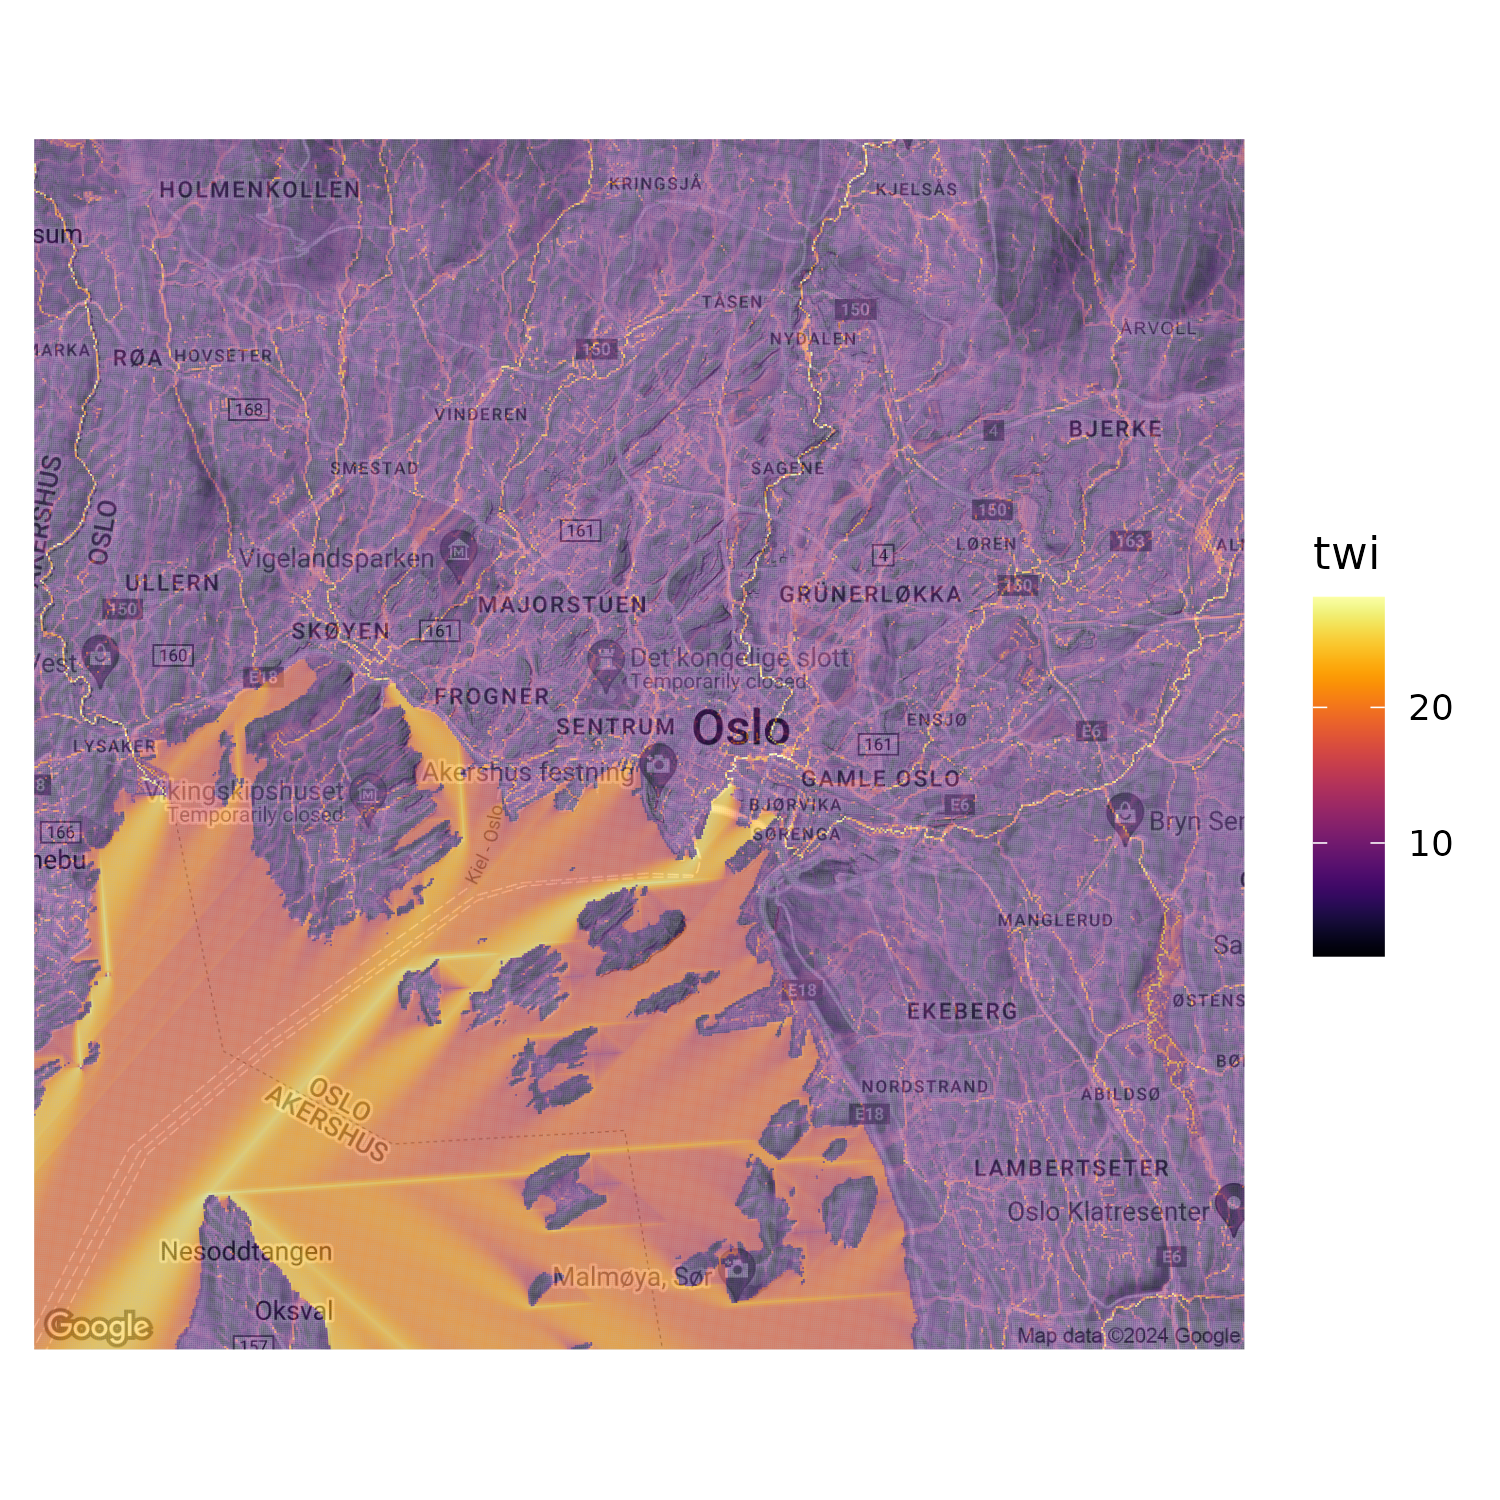
\includegraphics[
        width=\linewidth,
        height=0.50\textheight,
        keepaspectratio,
        trim={0 125 0 55},
        clip
      ]{images/data/example_plot_twi.png}

      \raisebox{-0.1cm}[0pt][0pt]{%
        % \footnotesize High values: drainage paths and flat areas%
        \footnotesize High values: flat and/or large upslope area%
      \framefootcitecompact{Mattivi&2019}}
    \end{column}
    \begin{column}{0.49\textwidth}
      \centering
      \hspace{-0.4cm}
      Height above nearest drainage (HAND)\\[0.08cm]
      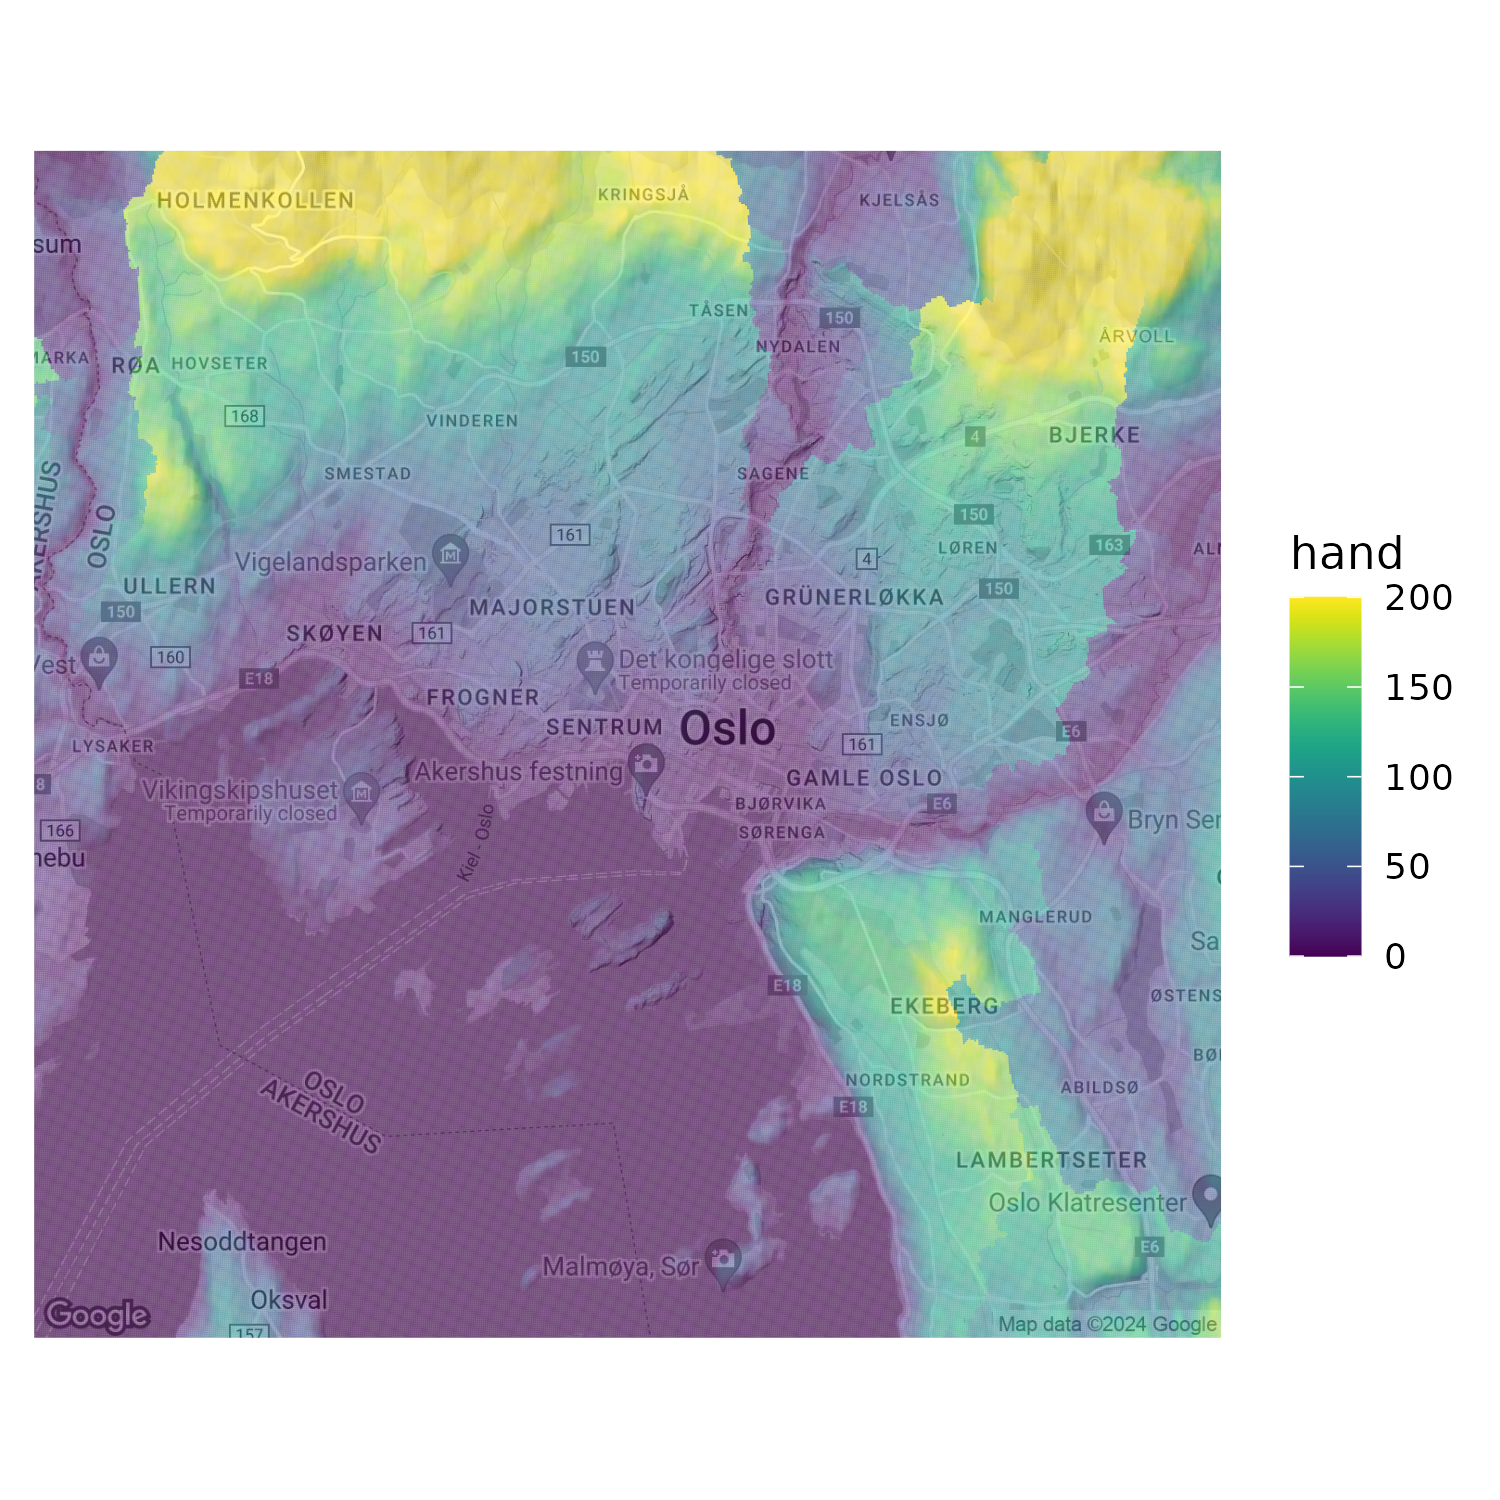
\includegraphics[
        width=\linewidth,
        height=0.50\textheight,
        keepaspectratio,
        trim={0 125 0 55},
        clip
      ]{images/data/example_plot_hand.png}\\
      \raisebox{-0.1cm}[0pt][0pt]{%
        \footnotesize High values: elevated from drainage%
      \framefootcitecompact{Nobre&2011}}
    \end{column}
  \end{columns}
  \vspace{0.5cm}
  \footnotesize
  \textbf{Land use:} reduced to binary categories
  \emph{urban} versus \emph{non-urban}%
  \framefootcitecompact{nibio_ar50_docs}
\end{frame}

\begin{frame}{Extreme precipitation measures}
  \vspace{0.5cm}
  \begin{columns}[T,onlytextwidth]
    \begin{column}{0.46\textwidth}
      \textbf{Daily precipitation}
      \begin{itemize}
        \item Historical seNorge observations on a 1 x 1 km$^2$
          grid\framefootcitecompact{lussana2020senorgeobservationalgriddeddatasets}
        \item Climate simulations from the Norwegian Centre for Climate
          Services\framefootcitecompact{Dyrrdal2025}
        \item Values linked to each insured building by location
      \end{itemize}
    \end{column}
    \begin{column}{0.49\textwidth}
      \textbf{Two aggregation scales}
      \begin{itemize}
        \item \textbf{Season-year:} daily values aggregated into indices
          measuring extreme precipitation
        \item \textbf{30-year reference:} local precipitation summaries
          describing the prevailing climate
      \end{itemize}

      \vspace{0.15cm}
      \footnotesize
      Constructed 11 season-year indices, three 30-year reference measures.
    \end{column}
  \end{columns}
\end{frame}

\begin{frame}{Static climate summaries to seasonal extremes}
  \vspace{0.5cm}
  \footnotesize
  Retain building-level GAM framework:\\
  Property, topographic, and regional effects similar to those in
  Heinrich-Mertsching et al.\framefootcitecompact{HeinrichMertsching2023}.

  \vspace{0.5cm}
  \begin{columns}[T,onlytextwidth]
    \begin{column}{0.38\textwidth}
      \textit{Previous model:}
      \begin{itemize}
        \item Static climate summaries over a 30-year period
        \item Mean daily precipitation
        \item Mean temperature
      \end{itemize}
    \end{column}
    \begin{column}{0.57\textwidth}
      \textit{This project: season-year extremes}
      \begin{enumerate}
        \item \textit{Absolute intensity}\newline
          % Mean of the three wettest daily precipitation totals in
          % each season-year
          Measure of maximum daily precipitation in each season-year
        \item \textit{Relative intensity}\newline
          % \textit{Absolute intensity} relative to the local 95th
          % percentile of daily precipitation
          \textit{Absolute intensity} relative to high local
          quantile of daily precipitation
      \end{enumerate}
    \end{column}
  \end{columns}
\end{frame}
